% !TEX root = ../MasterThesis_goto_v1.tex

%%%%%%%%%%%%%%%%%%%%%%%%%%%%%%%%%%%%%%%%%%%%%%%%%%%%%%%%%%%%%%%%%%%%%%%%%%%%%%%%%%%%%%%%%%%%%%%%%%%%%
\chapter{序論} \label{chap:Introduction}

本章では、まず\ref{Intro:StandardModel}節で素粒子を記述する為の理論である、標準模型 (Standard Model, SM) について解説する。
次に、この標準模型や標準模型を超える物理 (Physics beyond the Standard Model, BSM) を探索するための国際線形加速器 (International Linear Collider, ILC) 計画についての説明を\ref{Intro:InternationalLinearColliderProject}節で行う。
また、このILCで観測できる主な物理現象については\ref{Intro:PhysicsofILC}節で述べる。
ILCの検出器は、International Large Detector (ILD) とSilicon Detector (SiD) の二つが検討されている。
本研究はILDに関する研究である為、ILDについて\ref{Intro:InternationalLargeDetector}節で簡単に説明する。
ただし、本研究の基本的な構想はそのような検出器に寄らず使用できる。

加速器実験では、取得したデータをそのまま物理解析に使用することは出来ず、適切な処理をする必要があり、これを事象再構成 (Event Reconstruction) という。
\ref{Intro:SoftwareandEventReconstructionofILC}節では、ILCにおけるこれら再構成手法やソフトウェアについて説明し、最後に本研究の目的について\ref{Intro:Purpose}節で述べ、本論文の序論とする。

%%%%%%%%%%%%%%%%%%%%%%%%%%%%%%%%%%%%%%%%%%%%%%%%%%%%%%%%%%%%%%%%%%%%%%%%%%%%%%%%%%%%%%%%%%%%%%%%%%%%%
\section{標準模型} \label{Intro:StandardModel}

宇宙の誕生や、生物の発生と同様に、物質の起源は人類の根元的な問いの一つである。
そのような物質の素となる粒子のことを素粒子といい、その素粒子の振る舞いを記述する理論を標準模型という。
この標準模型は20世紀から多数の物理学者によって構築され、今日に至るまで様々な実験によって、非常に良く確かめられている。
標準模型によると、素粒子はスピン半整数のフェルミ粒子とスピン整数のボース粒子に分類される。

フェルミ粒子は全てスピン$1/2$の粒子で構成され、更に、陽子や中性子などを構成するクォークと電子やニュートリノなどのレプトンに分けられる。
クォークは電荷が$+2/3$のアップクォーク系列と$-1/3$のダウンクォーク系列に、レプトンは電荷が$-1$の荷電レプトンと中性電荷の中性レプトンに細分される。
また、それぞれ世代と呼ばれるものを構成し、現在合計で3つの世代が確認されている。
クォークの場合はアップクォーク$u$、チャームクォーク$c$、トップクォーク$t$、ダウンクォーク$d$、ストレンジクォーク$s$、ボトムクォーク$b$が存在し、これらの系列や世代間のクォークの違いをフレーバーと呼んでいる。レプトンの場合は荷電レプトンとして、電子$e^-$、ミュー粒子$\mu^-$、タウ粒子$\tau^-$、中性レプトンとして、電子ニュートリノ$\nu_e$、ミューニュートリノ$\nu_{\mu}$、タウニュートリノ$\nu_{\tau}$が存在している。

ボース粒子は基本的な4つの力である、強い相互作用、弱い相互作用、電磁相互作用、重力相互作用の内、重力相互作用を除いた3つの力をそれぞれ媒介するスピン1のゲージ粒子と、対称性を破り素粒子に質量を与えるスピン0、中性電荷のヒッグス粒子$H$で構成される。
電磁相互作用を媒介する粒子として、中性電荷の光子$\gamma$、強い相互作用を媒介する粒子として、中性電荷のグルーオン$g$、弱い相互作用を媒介する粒子として、電荷$\pm 1$のWボソン$W^{\pm}$、中性電荷のZボソン$Z$が存在する。


粒子には、質量やスピンが等しく、電荷の正負が反転した反粒子が存在し、基本的にそれぞれの粒子に$\bar{}$や電荷をつけて記述される。 ($\bar{u}, \bar{c}, \bar{t}, \bar{d}, \bar{s}, \bar{b}, e^+, \mu^+, \tau^+, \bar{\nu}_{e}, \bar{\nu}_{\mu}, \bar{\nu}_{\tau}$)
これらの反粒子と通常の粒子を衝突させると、質量が全てエネルギーへと変換される、対消滅を起こす。
一方、これらの粒子対以上のエネルギーを与えた場合は対生成が起こり、これらの粒子対が生成される。

これらのボース粒子、フェルミ粒子は標準模型の素粒子と呼ばれ、一般に図\ref{1SMParticle}のように纏められている。

\begin{figure}[htbp]
 \centering
 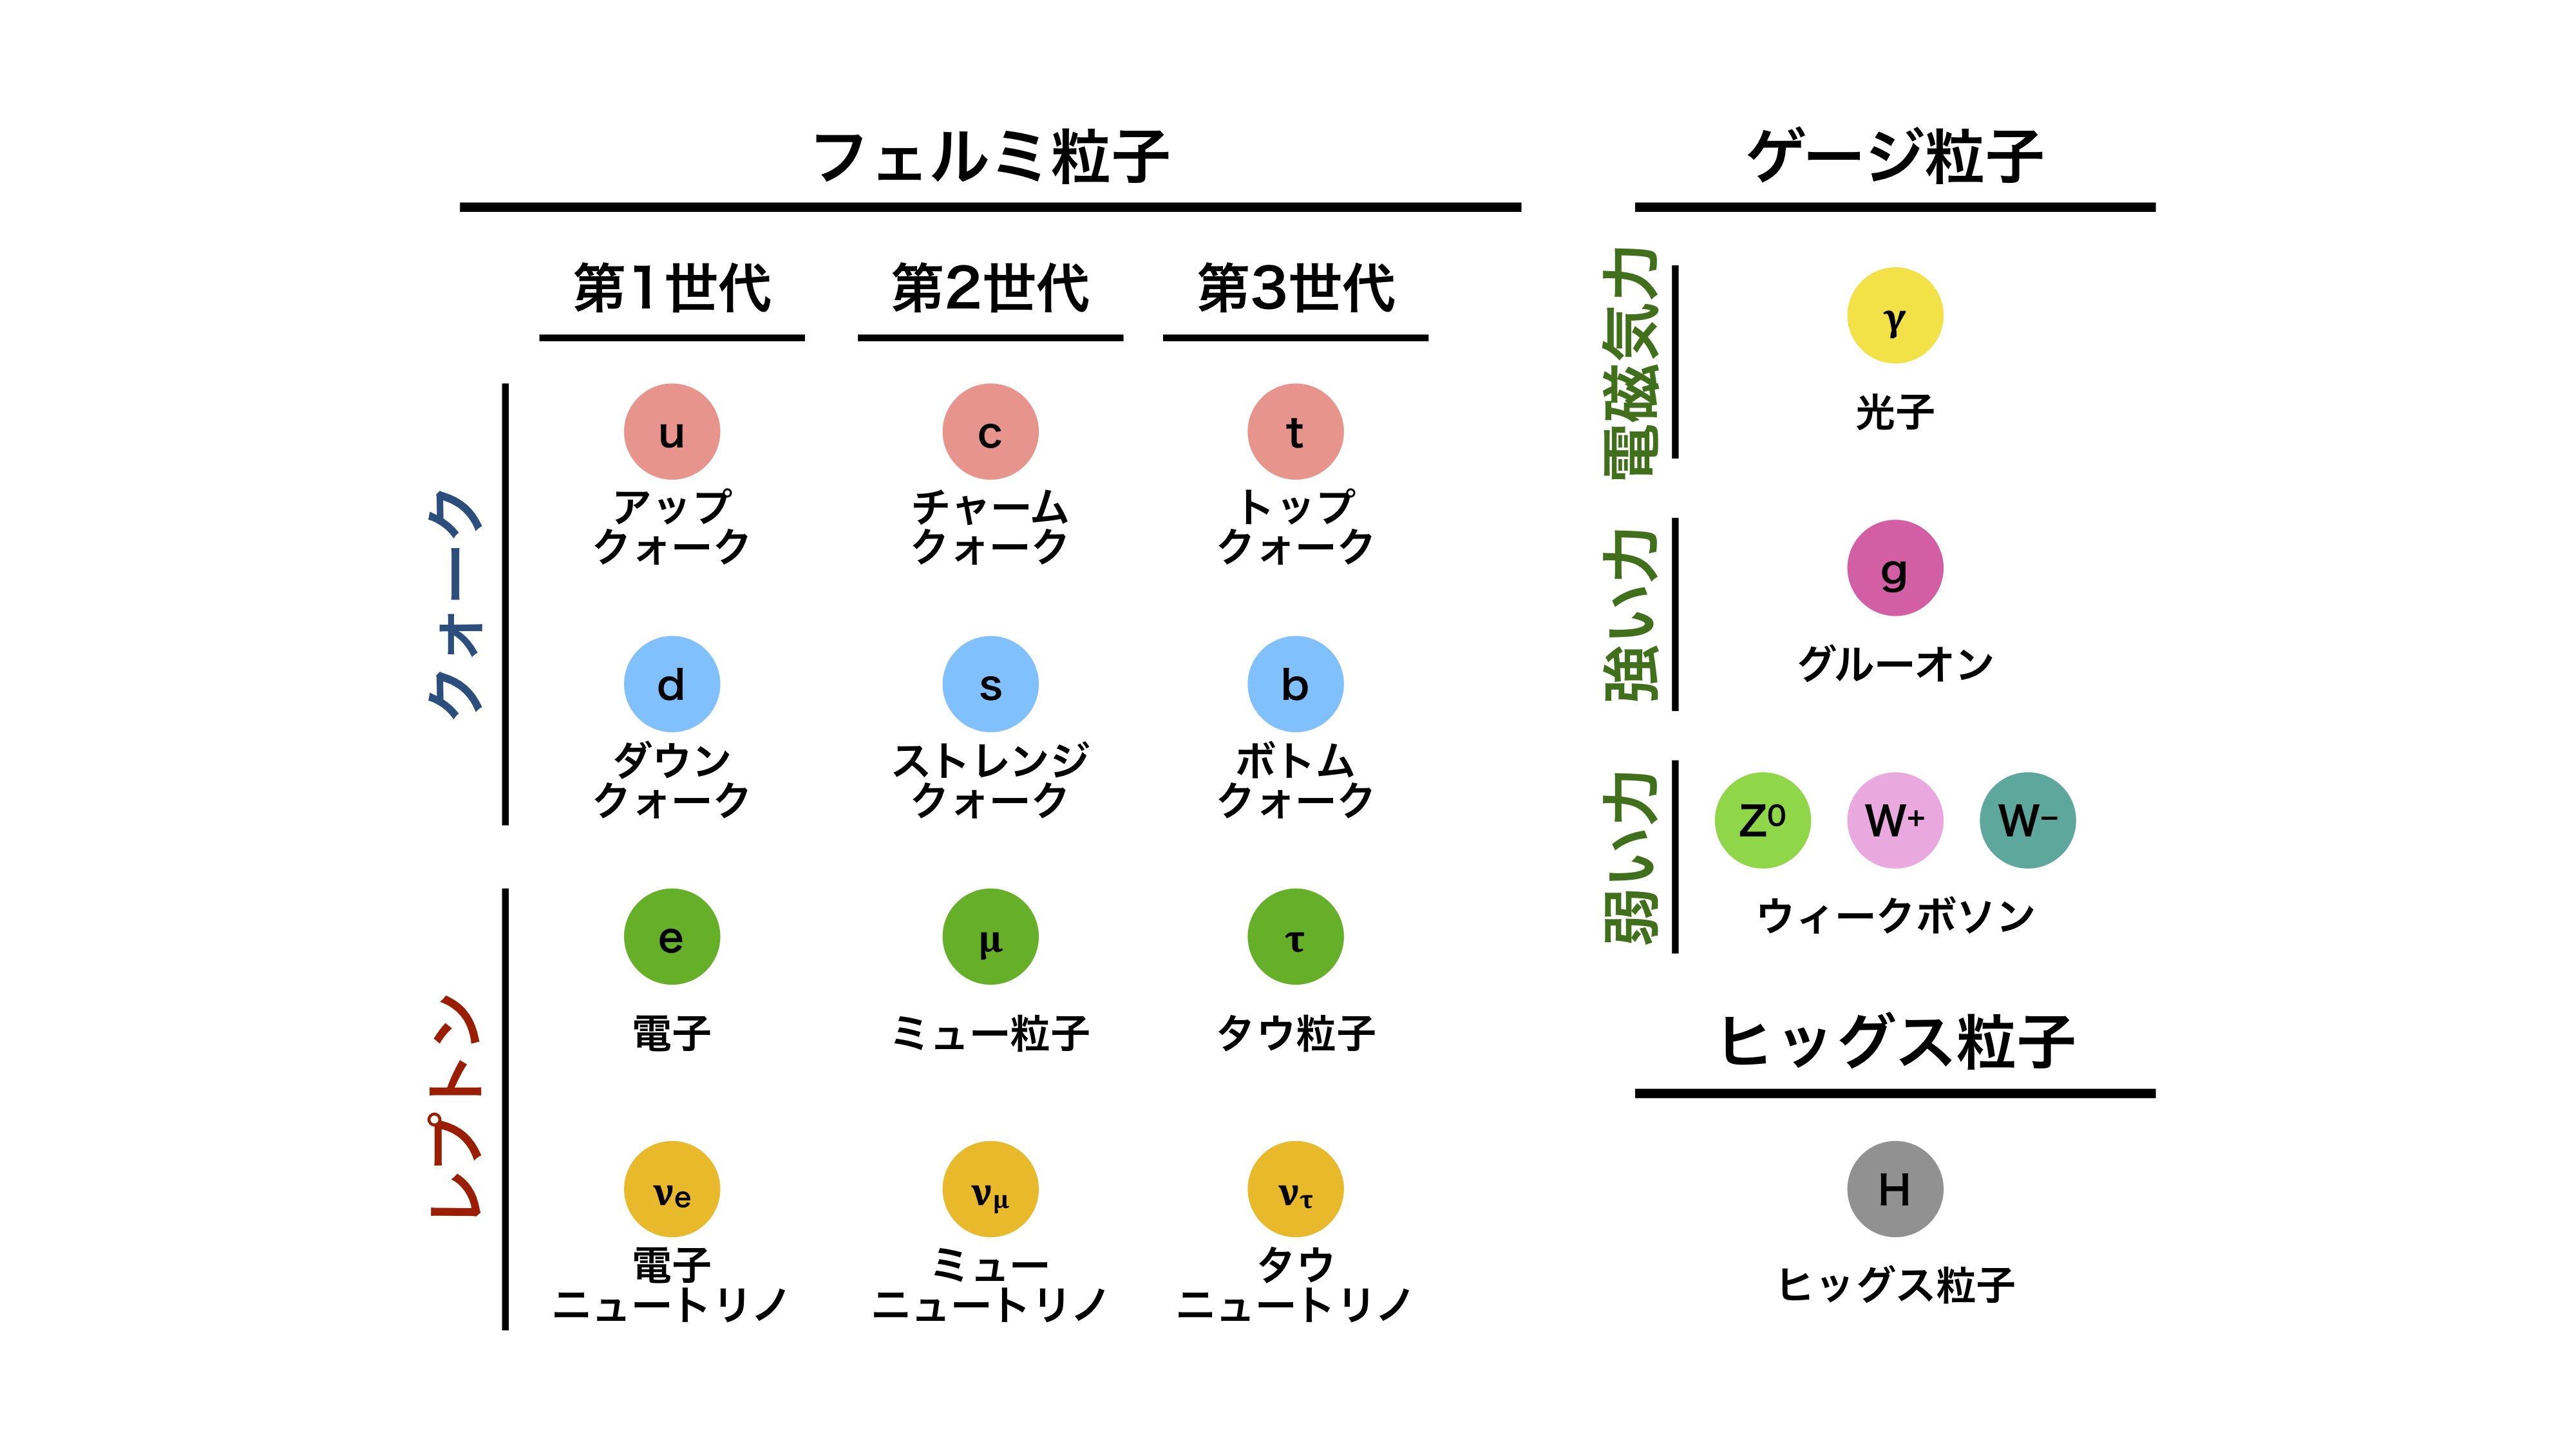
\includegraphics[width=0.9\textwidth]{Figure/1Introduction/1SMParticle.png}
 \caption{標準模型の素粒子}
 \label{1SMParticle}
\end{figure}

前述したように、標準模型は様々な実験で非常によく確かめられているが、ダークマターをはじめとするいくつかの物理現象を説明できておらず、現在は様々な実験によって、BSMの探索が行われている。
次節のILC計画はそのような試みの一つである。

%%%%%%%%%%%%%%%%%%%%%%%%%%%%%%%%%%%%%%%%%%%%%%%%%%%%%%%%%%%%%%%%%%%%%%%%%%%%%%%%%%%%%%%%%%%%%%%%%%%%%
\section{国際線形加速器 (ILC) 計画} \label{Intro:InternationalLinearColliderProject}

ILC計画とは、日本の東北にある北上山地に全長20.5kmの国際線形加速器 (ILC) を建設する計画である。 (図\ref{2InternationalLinearCollider})
ILC計画は国際共同研究であり、2013年に出版されたThe Technical Design Report (TDR)には2400人の研究者、48の国と392の研究機関と大学のグループが著名している。
このILC実現の為の技術開発はリニアコライダーコラボレーション (The Linear Collider Collaboration, LCC) によって推進され、LCCの活動は国際将来加速器委員会 (The International Committee for Future Accelerator, ICFA) の下、リニアコライダー国際推進委員会 (Linear Collider Board, LCB)によって監督されている。
現在ILC計画は準備段階へ向けて計画が進められており、日本のILC準備研究所 (ILC Pre-Lab) の為の準備としてICFAはILCの国際推進チーム (International Development Team, IDT) の設立を承認した。
今後はLCCやLCBに代わり、このILC国際推進チームがILC計画の推進を行なっていく予定である。
ILC計画の今後の流れは図\ref{3ILCProject}に示している。

\begin{figure}[htbp]
 \centering
  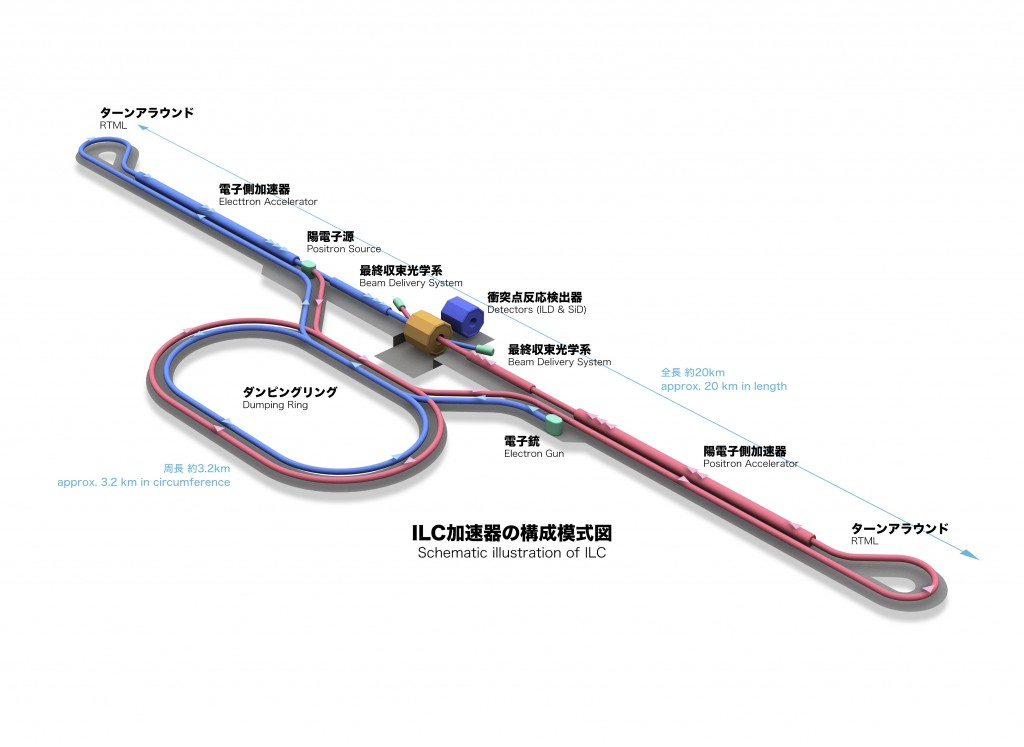
\includegraphics[width=0.9\textwidth]{Figure/1Introduction/2InternationalLinearCollider.jpg}
  \caption{国際線形加速器 (ILC) の外観\cite{ILCPHOTO}}
  \label{2InternationalLinearCollider}
\end{figure}


\begin{figure}[htbp]
 \centering
 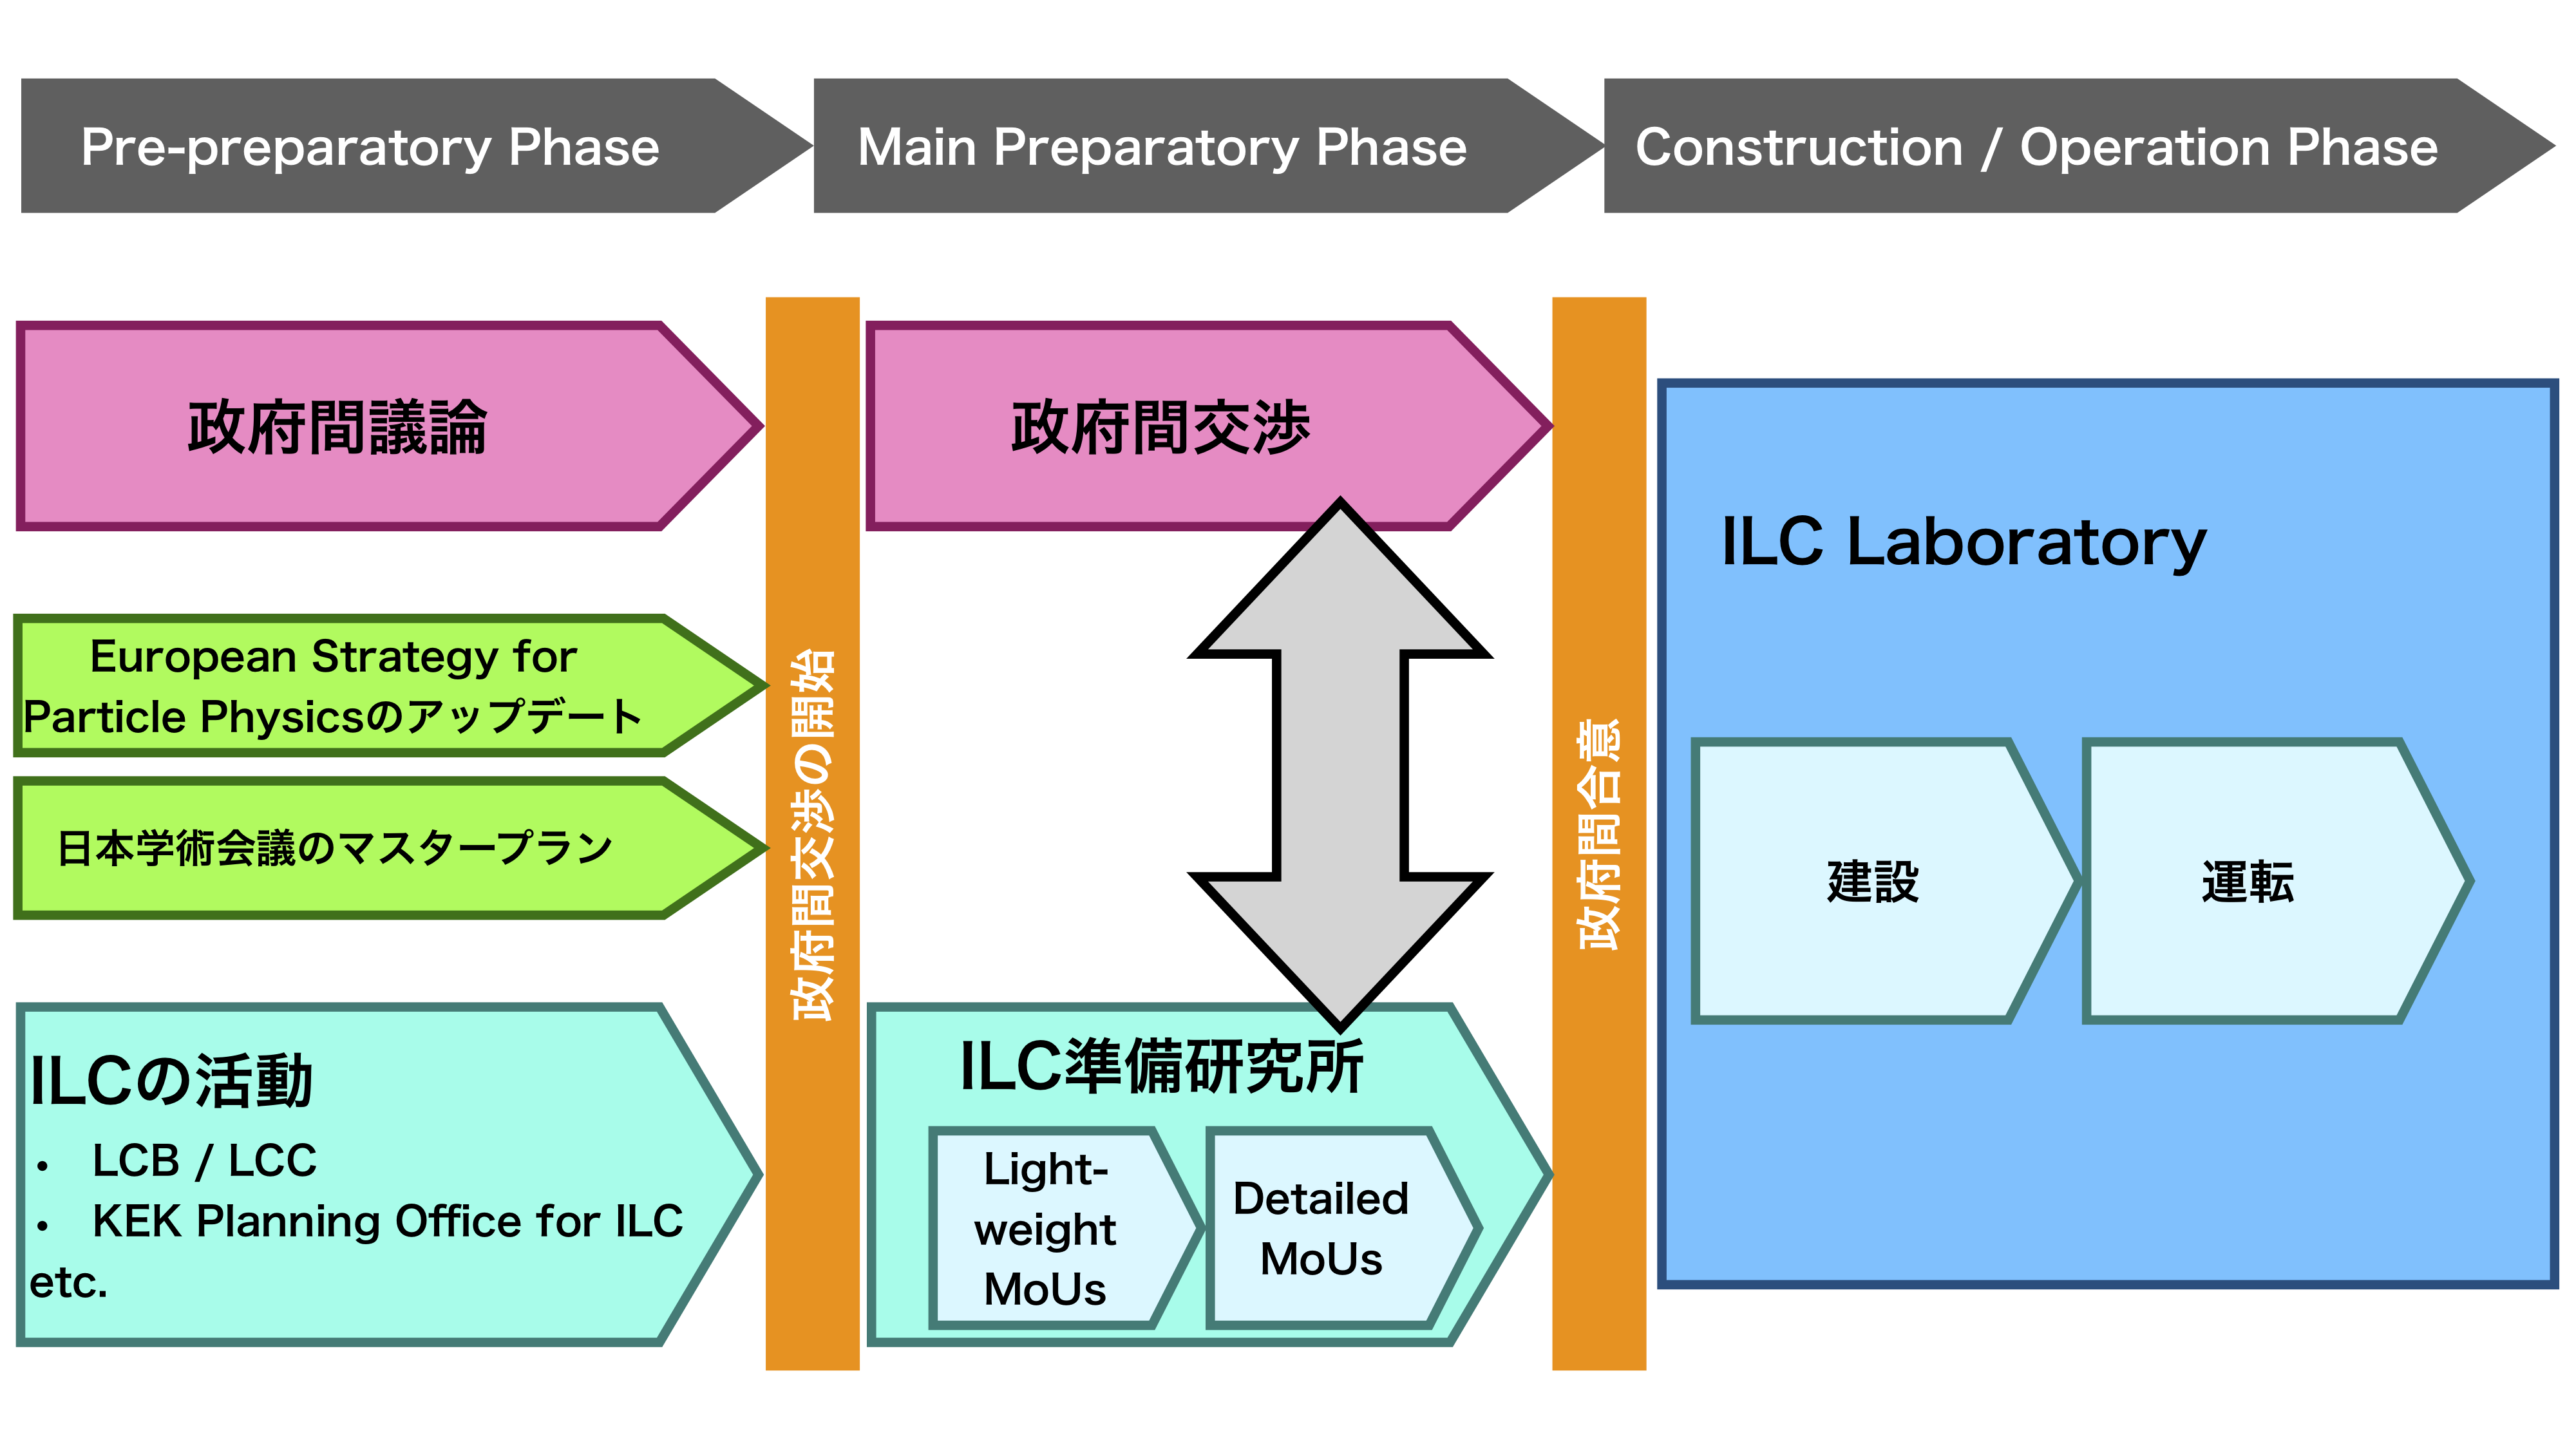
\includegraphics[width=0.9\textwidth]{Figure/1Introduction/3ILCProject.png}
 \caption{ILC計画の今後\cite{RecommendationsonILCProjectImplementation}}
 \label{3ILCProject}
\end{figure}

%%%%%%%%%%%%%%%%%%%%%%%%%%%%%%%%%%%%%%%%%%%%%%%%%%%%%%%%%%%%%%%%%%%%%%%%%%%%%%%%%%%%%%%%%%%%%%%%%%%%%
\section{ILCの物理} \label{Intro:PhysicsofILC}

ヒッグス粒子が2012年に欧州原子核研究機構(CERN)の大型ハドロン衝突型加速器(Large Hadron Collider, LHC)で発見されて以降、ヒッグス粒子の性質について、より詳細な調査が行われている。
ヒッグス粒子は標準模型の中で、電弱相互作用の対称性を破り、素粒子に質量を与える役割を担っており、また、質量に結合するという特徴を持っている。
このような振る舞いからヒッグス粒子の性質は標準模型によって詳細に決定される為、BSMによって標準模型との差異が生じた場合、ヒッグス粒子はその影響を受けると予想されている。
特にヒッグス粒子と他の粒子との結合定数の変化は、そのような仮定するBSMの模型の違いによって異なることが示唆されている。

ILCはこのヒッグス粒子の性質を詳細に調べる為のヒッグスファクトリーとしての役割を期待されている。
LHCが陽子-陽子衝突であるのに対し、ILCは電子-陽電子を衝突させる加速器である。
したがって、粒子反粒子の関係となっており、目的とする事象に対しエネルギーをより効率的に使うことができる。
また、電子-陽電子は陽子同士の衝突と異なり、背景事象が少ないという特徴を持っている。

ILCは$e^+e^- \to Zh$事象の反応断面積が最大となる重心系エネルギー$\sqrt{s}=250\ \mathrm{GeV}$での運転開始 (ILC250) を予定している。(図\ref{4eetoZH})
また、ILCには様々な物理目標を達成する為に多数のアップグレードオプションが存在し、重心系エネルギーについてはメインリニアックを延長することで$1\ \mathrm{TeV}$までの拡張が可能である。

\begin{figure}[htbp]
 \centering
 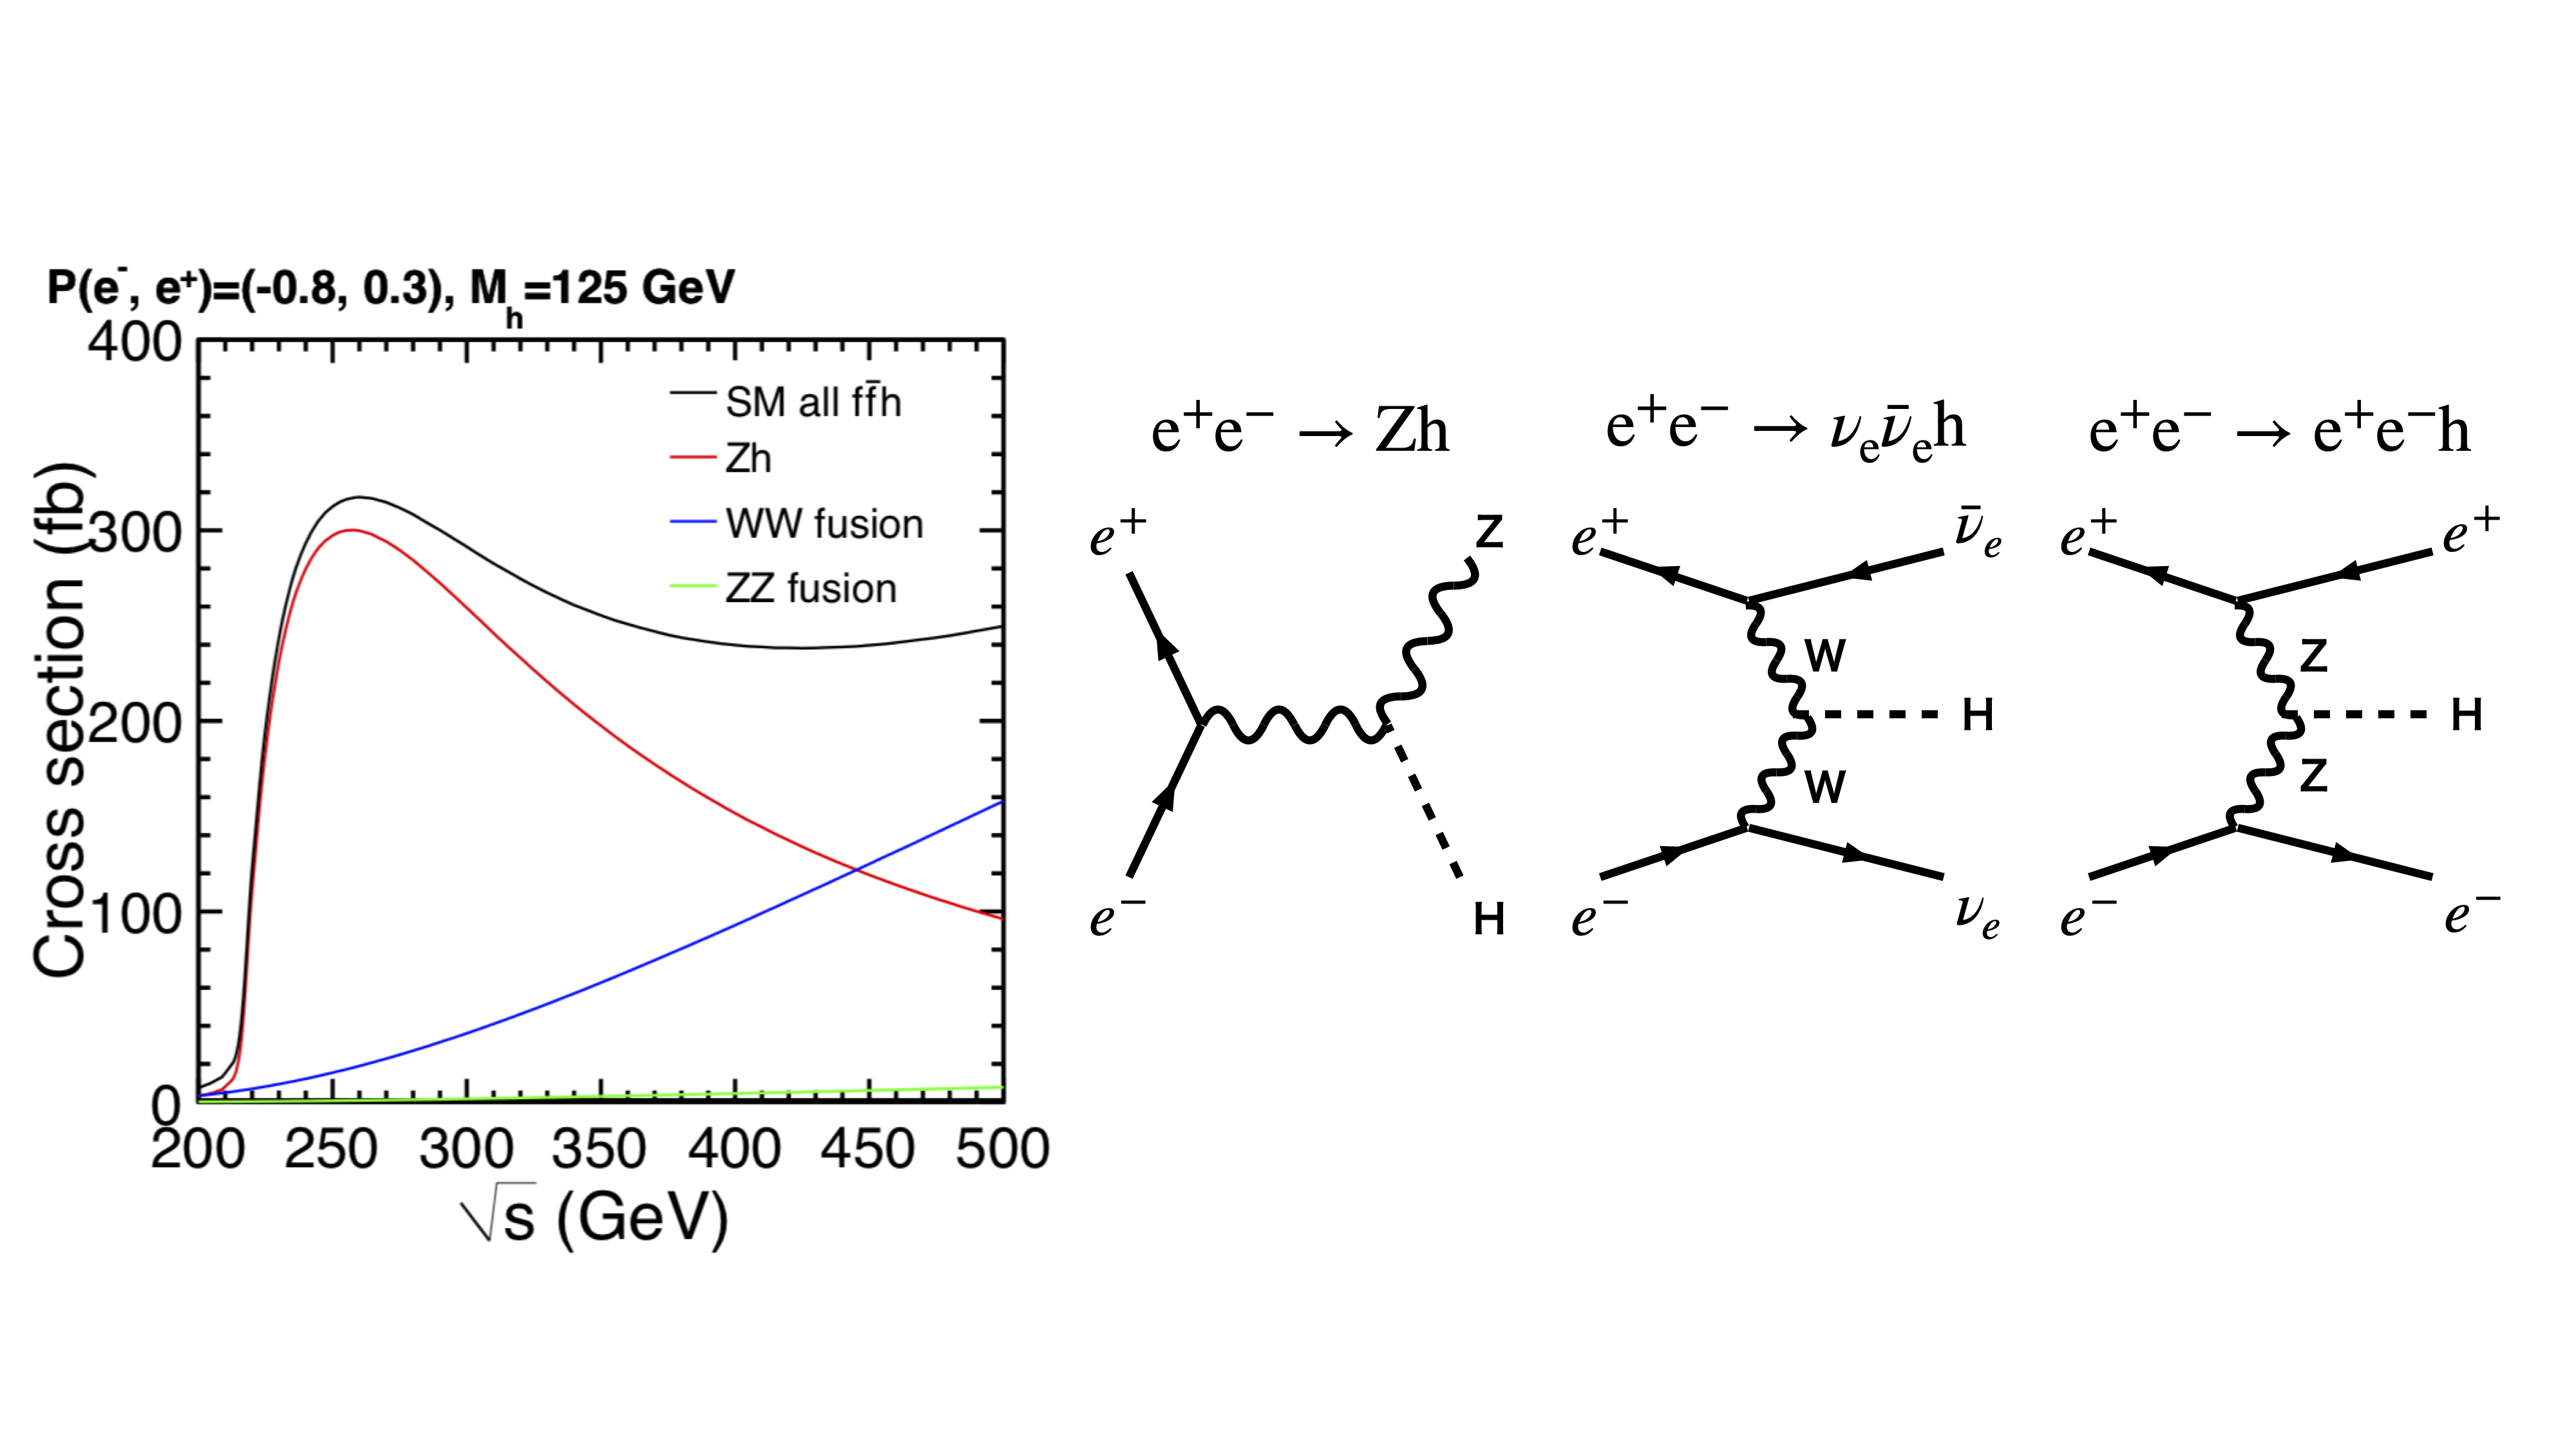
\includegraphics[width=0.7\textwidth]{Figure/1Introduction/4eetoZH.png}
 \caption{重心系エネルギーと生成断面積の関係\cite{TechnicalDesignReportPhysics}}
 % The International Linear Collider Technical Design Report - Volume 2: Physics Fig 2.7
 \label{4eetoZH}
\end{figure}

$e^+e^- \to Zh$事象は$Z$粒子の識別をすることによって、ヒッグスの崩壊モードに寄らず事象を選別できる (リコイル) という点で非常に重要である。
また、背景事象である$e^+e^- \to Z\gamma$や$e^+e^- \to ZZ$に関してもよく理解されており、電弱相互作用の計算によって$0.1\ \%$程度に抑えることができる。\cite{GlobalProject}
したがって、$e^+e^- \to Zh$事象の全断面積を得ることができ、絶対正規化されたヒッグス粒子の結合定数やヒッグス粒子のエキゾチック崩壊についての測定が可能である。

$e^+e^- \to Zh$事象での終状態の$Z$粒子は、レプトン対またはクォーク対に崩壊する。
レプトン対にはおよそ30\%程度の割合で崩壊し、クォーク対には残りの70\%程度の割合で崩壊する為、統計量を大きくするという点でクォーク対をより精度よく識別することは非常に重要である。
これらのクォーク対はエネルギー効率のために、それぞれ真空中でクォークの粒子反粒子対を生成・結合しハドロンとなる。
この過程で生成されたクォークも同様にハドロンを形成するため、初めのクォーク対のそれぞれの進行方向には多数のハドロン粒子が生成されることとなる。
これをジェットといい、$Z$粒子を始めとする様々な粒子のクォーク対への崩壊は、このジェットを用いて識別される。
そのようなジェットの再構成については、\ref{Intro:SoftERILC:JetReconstruction}項にて説明する。

%%%%%%%%%%%%%%%%%%%%%%%%%%%%%%%%%%%%%%%%%%%%%%%%%%%%%%%%%%%%%%%%%%%%%%%%%%%%%%%%%%%%%%%%%%%%%%%%%%%%%
\section{ILCの検出器 -International Large Detector (ILD)-} \label{Intro:InternationalLargeDetector}

ILCでは二つの検出器が検討されており、ILD(図\ref{5-1InternationalLargeDetector})はその一つである。
ILDはヒッグス粒子や電弱相互作用の物理からの要求値を満たすように設計され、また後述するParticle Flow (\ref{Intro:SoftERILC:ParticleReconstruction}項) によって最適化されている。
また、様々なサブディテクターによって構成され、ビームの衝突点 (図\ref{5-2InternationalLargeDetector}の右下) を包む様に内側から順に、Vertex Detector (VTX)、Silicon Internal Tracker (SIT)、Time Projection Chamber (TPC)、Electromagnetic Calorimeter (ECAL)、Hadron Calorimeter (HCAL)、Iron Yoke (Muon が並んでいる。
HCALとIron Yokeの間にはSolenoid Coilがあり、$3.5 \mathrm{T}$の磁場をかけている。
VTXやSIT、TPCを用いて荷電粒子の飛跡を測定し、ECALによって電子や光子などの粒子のエネルギーを、HCALによってハドロン粒子のエネルギーを測定する。
衝突点の前方方向には、Forward Tracking Detector (FTD)、Luminosity Calorimeter (LumiCAL)、LHCAL、Beam Calorimeter (BeamCAL)が並んでいる。
それぞれの技術的な詳細については表\ref{ILDSubdetectorParametersBarrel}、\ref{ILDSubdetectorParametersEndCap}にまとめる。

\begin{figure}[htbp]
 \centering
 \begin{minipage}{0.47\textwidth}
  \centering
  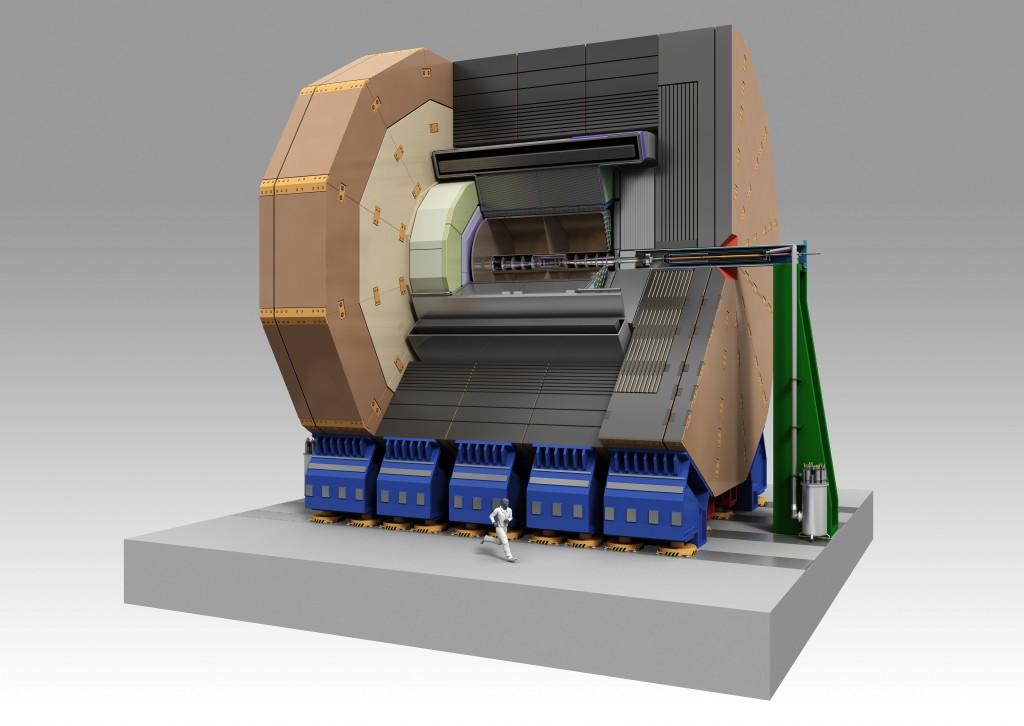
\includegraphics[width=1\textwidth]{Figure/1Introduction/5-1InternationalLargeDetector.jpg}
  \caption{外観\cite{ILCPHOTO}}
  \label{5-1InternationalLargeDetector}
 \end{minipage}
 \begin{minipage}{0.47\textwidth}
   \centering
   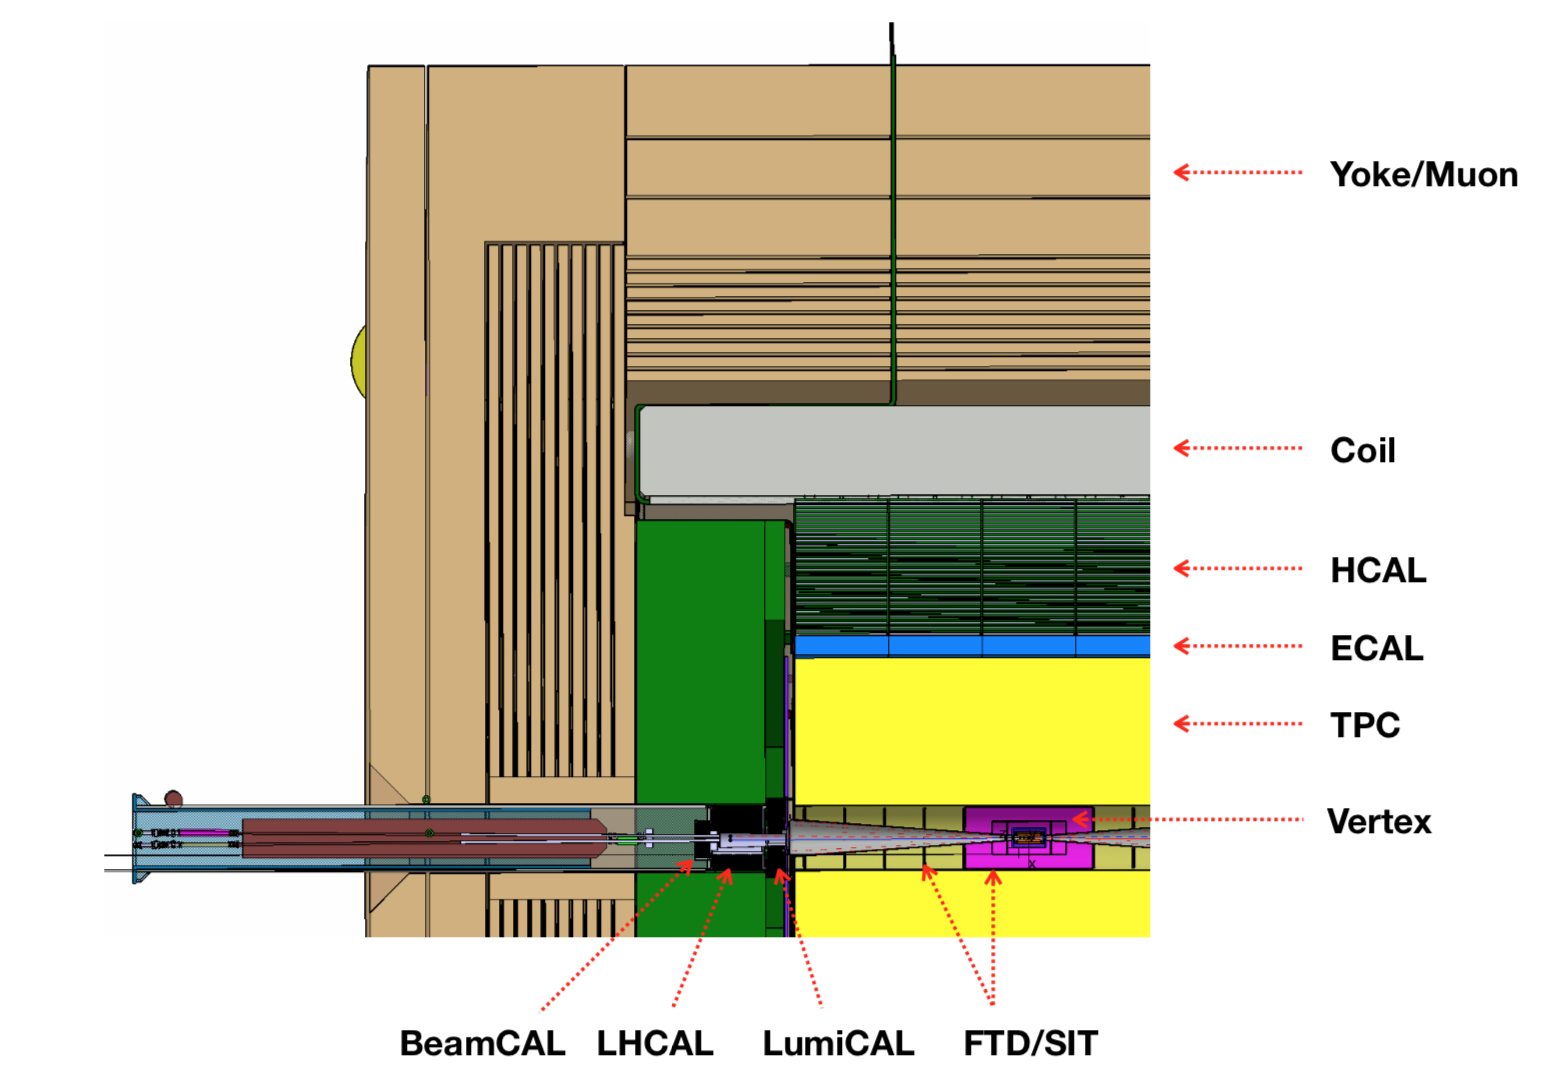
\includegraphics[width=1\textwidth]{Figure/1Introduction/5-2InternationalLargeDetector.png}
   \caption{縦断面\cite{InterimDesignReport}}
   \label{5-2InternationalLargeDetector}
    % INTERIM DESIGN REPORT Figure 5.1
 \end{minipage}
 \caption{International Large Detector (ILD)}
\end{figure}

\begin{table}[htb]
 \centering
  \small
  \begin{tabular}{l c c c l} \hline
     & $r_{in} \mathrm{[mm]}$ & $r_{out} \mathrm{[mm]}$ & $z_{max} \mathrm{[mm]}$ & 要素技術\\ \hline \hline
    VTX & 16 & 60 & 125 & シリコンピクセルセンサー\\
    SIT & 153 & 303 & 644 & シリコンピクセルセンサー\\
    TPC & 329 & 1770 & 2350 & マイクロパターンガス検出器\\
    SET & 1773 & 1776 & 2300 & シリコンストリップセンサー\\ \hline
    ECAL & 1805 & 2028 & 2350 & 吸収層 : タングステン\\
    &&&& センサー : シリコン/シンチレーター\\
    HCAL & 2058 & 3345 & 2350 & 吸収層 : スチール\\
    &&&& センサー : シンチレーター/RPCガス\\ \hline
    Coil & 3425 & 4175 & 3872\\
    Muon & 4450 & 7755 & 4047 & センサー : シンチレーター\\ \hline
  \end{tabular}
  \caption{ILDサブディテクターの詳細なパラメータ (バレル) \cite{InterimDesignReport}}
  \label{ILDSubdetectorParametersBarrel}
\end{table}

\begin{table}[htb]
 \centering
 \small
  \begin{tabular}{l c c c c l} \hline
     & $z_{min} \mathrm{[mm]}$ & $z_{max} \mathrm{[mm]}$ & $r_{in} \mathrm{[mm]}$ & $r_{out} \mathrm{[mm]}$ & 要素技術\\ \hline \hline
    FTD & 220 & 371 & & 153 & シリコンピクセルセンサー\\
            & 645 & 2212 & & 300 & シリコンストリップセンサー\\ \hline
    ECAL & 2411 & 2635 & 250 & 2096 & 吸収層 : タングステン\\
    &&&&& センサー : シリコン\\
    &&&&& センサー : シンチレーター\\
    HCAL & 2650 & 3937 & 350 & 3226 & 吸収層 : スチール\\
    &&&&& センサー : シンチレーター\\
    &&&&& センサー : RPCガス\\
    Muon & 4072 & 6712 & 350 & 7716 & センサー : シンチレーター\\ \hline
    BeamCAL & 3115 & 3315 & 18 & 140 & 吸収層 : タングステン\\
    &&&&& GaAs読み出し \\
    LumiCAL & 2412 & 2541 & 84 & 194 & 吸収層 : タングステン\\
    &&&&& センサー : シリコン\\
    LHCAL & 2680 & 3160 & 130 & 315 &吸収層 : タングステン\\ \hline
  \end{tabular}
  \caption{ILDサブディテクターの詳細なパラメータ (エンドキャップ) \cite{InterimDesignReport}}
  \label{ILDSubdetectorParametersEndCap}
\end{table}

%%%%%%%%%%%%%%%%%%%%%%%%%%%%%%%%%%%%%%%%%%%%%%%%%%%%%%%%%%%%%%%%%%%%%%%%%%%%%%%%%%%%%%%%%%%%%%%%%%%%%
\section{ILCのソフトウェアと事象再構成} \label{Intro:SoftwareandEventReconstructionofILC}

ここではILCで使用されるソフトウェアと事象再構成について述べる。
ILCのソフトウェアはiLCSoft\cite{iLCSoft}と呼ばれるソフトウェアエコシステムにまとめられている。
ILCにおける事象再構成は、トラッキングやParticle Flowといった\ref{Intro:SoftERILC:ParticleReconstruction}. 粒子の再構成と、更にそれらによって再構成された粒子を使いジェットを再構成する\ref{Intro:SoftERILC:JetReconstruction}. ジェットの再構成に分けられる。
ILCではジェットの再構成は崩壊点検出、ジェットクラスタリング、フレーバータギングという行程に分けられる。
これらジェットの再構成はiLCSoft内のLCFIPlus\cite{LCFIPlus}によって行われている。

%%%%%%%%%%%%%%%%%%%%%%%%%%%%%%%%%%%%%%%%%%%%%%%%%%%%%%%%%%%%%%%%%%%%%%%%
\subsection{ソフトウェア} \label{Intro:SoftERILC:Software}

書く事\\
LCIO・Marlin・DD4hep\\


%%%%%%%%%%%%%%%%%%%%%%%%%%%%%%%%%%%%%%%%%%%%%%%%%%%%%%%%%%%%%%%%%%%%%%%%
\subsection{飛跡の再構成} \label{Intro:SoftERILC:ParticleReconstruction}

書く事\\
トラッキング・Particle Flow\\

%%%%%%%%%%%%%%%%%%%%%%%%%%%%%%%%%%%%%%%%%%%%%%%%%%%%%%%%%%%%%%%%%%%%%%%%
\subsection{ジェットの再構成} \label{Intro:SoftERILC:JetReconstruction}

書く事\\
トラッキング・Particle Flowを経て再構成された粒子の飛跡を用いて、ジェットの再構成が行われる。
粒子が飛んでーーーーprimary vertexとsecondary vertex (崩壊点) を形成する\\
secondary vertexはジェットの種であり、これを検出するアルゴリズムを崩壊点検出といい、その様にして検出されたsecondary vertexを用いて、中性電荷を合わせた飛跡について、どのジェットに属するかクラスタリングを行うアルゴリズムをジェットクラスタリングという。
また、secondary vertexによってーーーーをフレーバータギングという。
以上がジェットの再構成である。
ここでは、LCFIPlus\cite{LCFIPlusPaper}でのジェット再構成手法についてまとめる。

まず、Primary Vertex

次に、Secondary Vertex

ジェットクラスタリング・Durham

フレーバータギング・Boosted Decision Trees (BDTs)

%%%%%%%%%%%%%%%%%%%%%%%%%%%%%%%%%%%%%%%%%%%%%%%%%%%%%%%%%%%%%%%%%%%%%%%%%%%%%%%%%%%%%%%%%%%%%%%%%%%%%
\section{本研究の目的} \label{Intro:Purpose}

\begin{figure}[htbp]
 \centering
 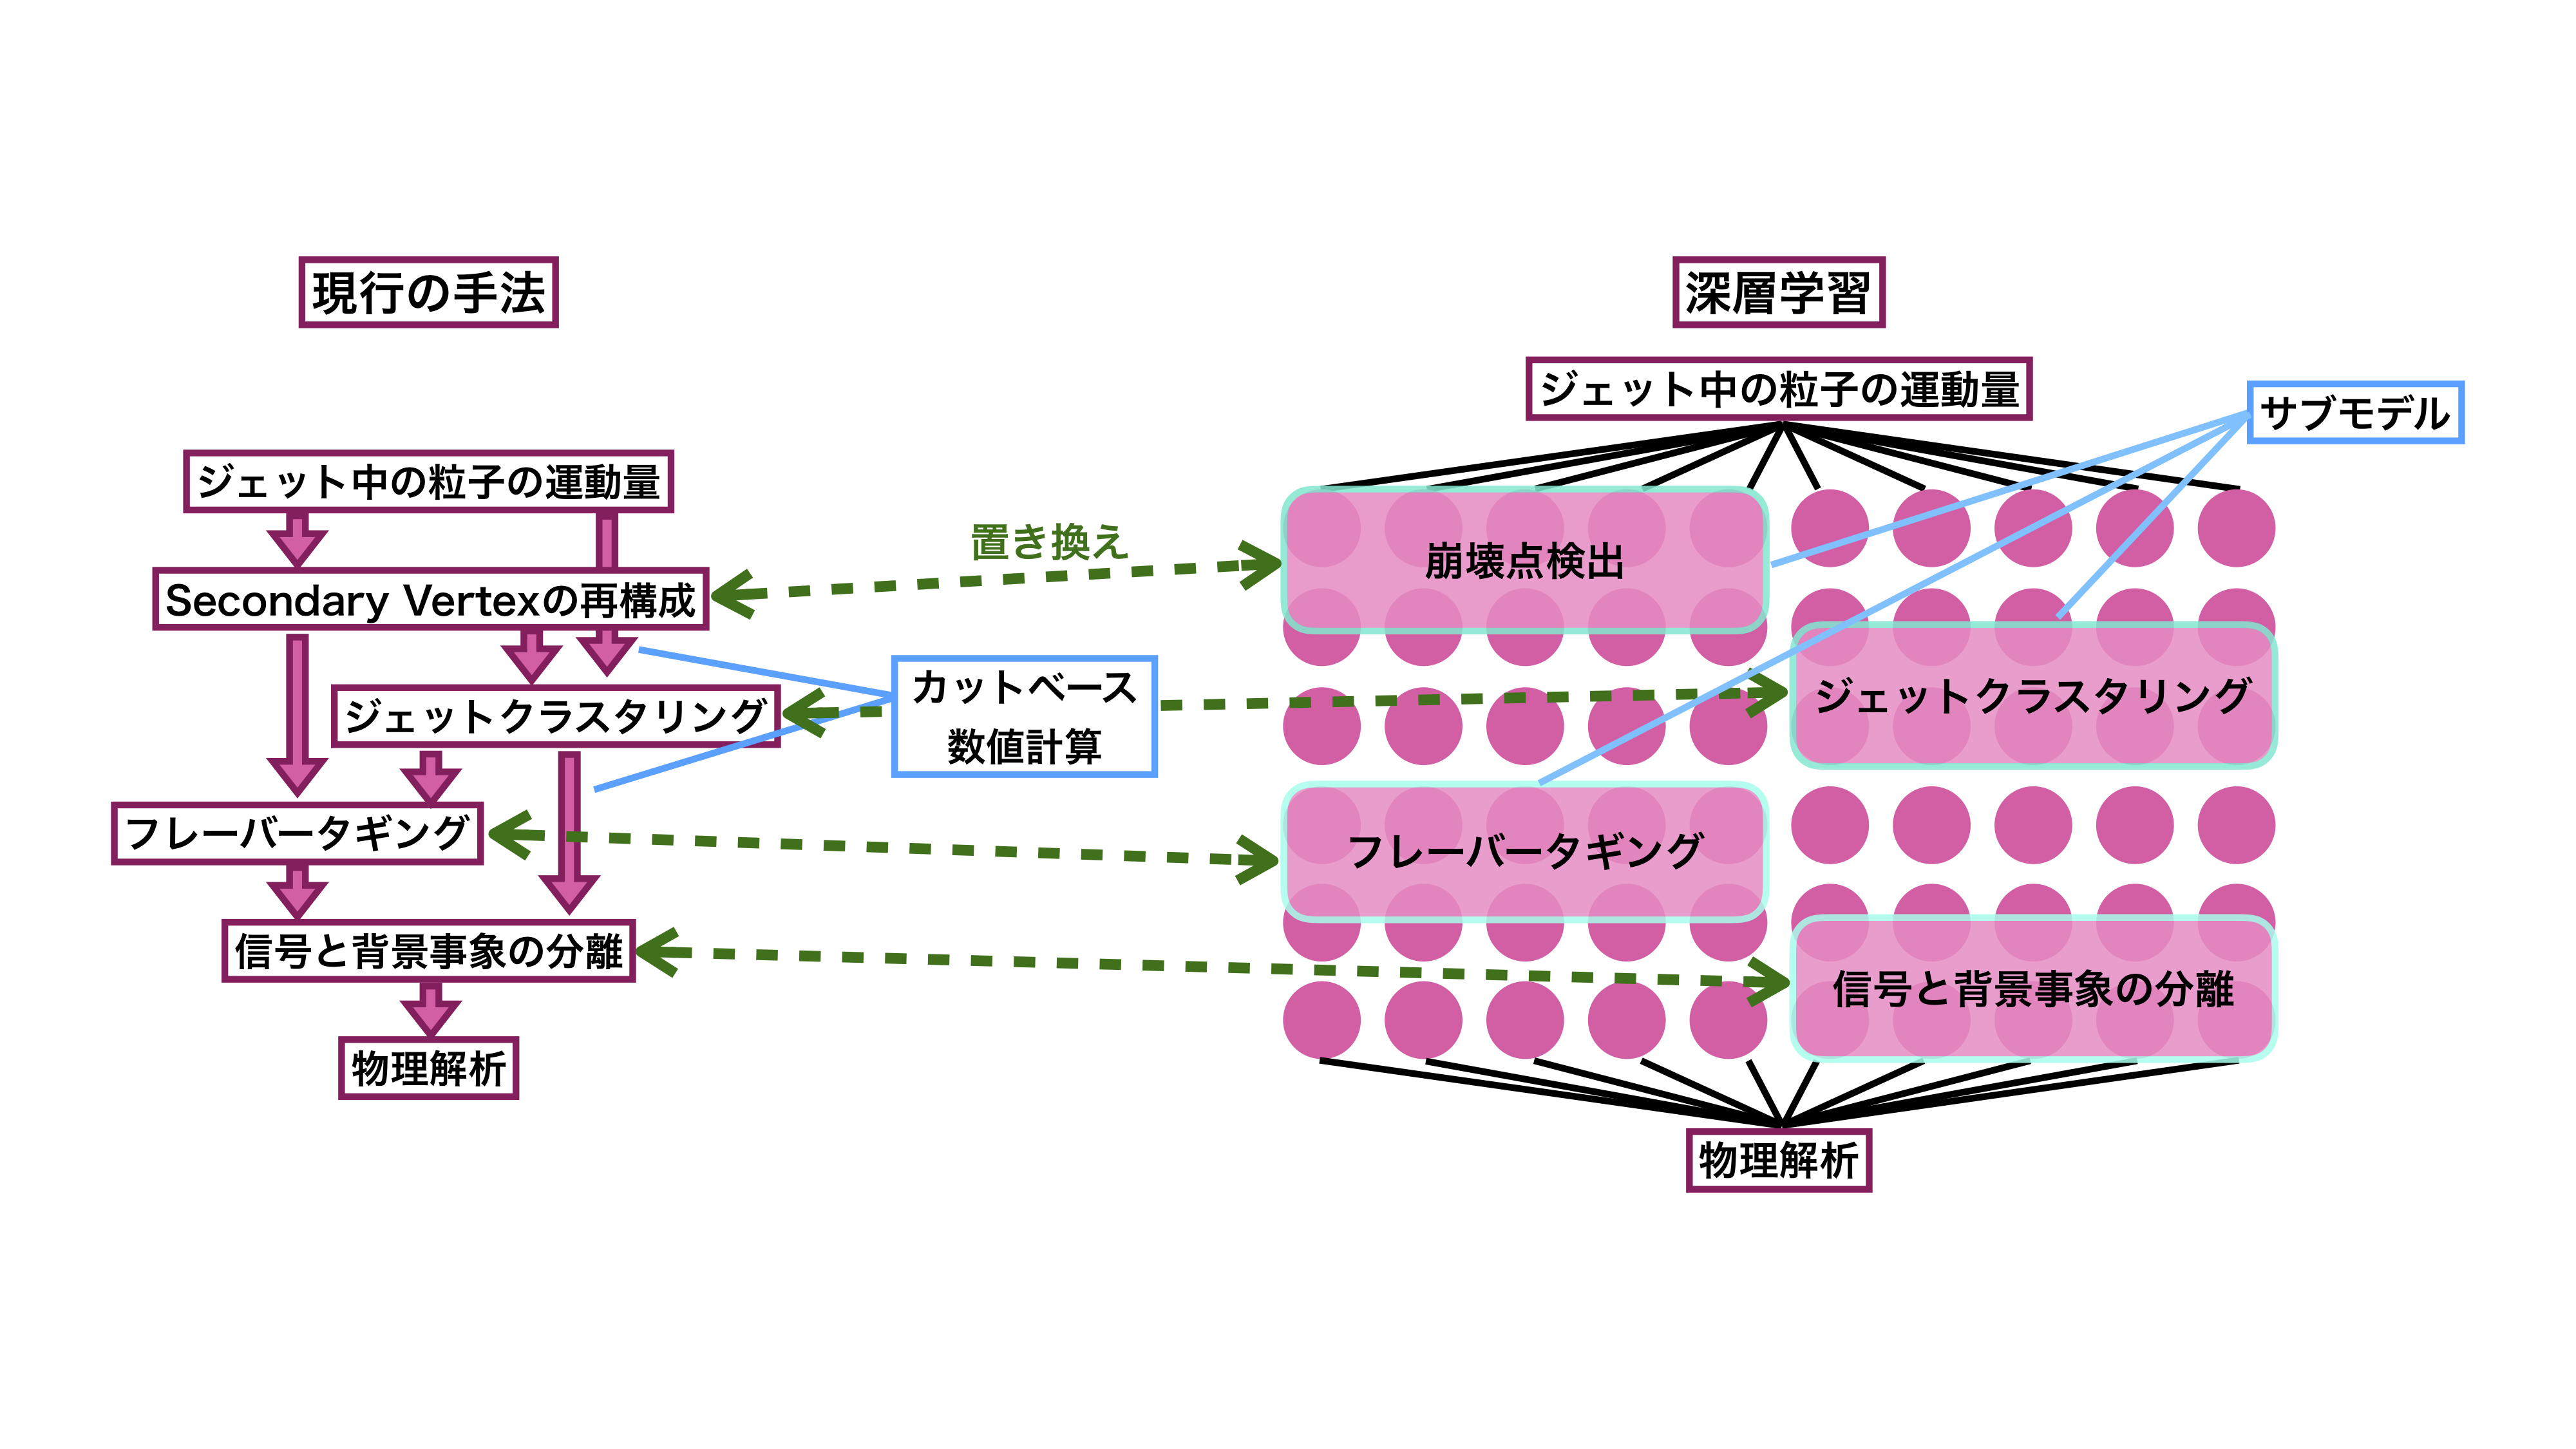
\includegraphics[width=1.0\textwidth]{Figure/1Introduction/6JetReconstructionwithDeepLearning.png}
 \caption{深層学習によるジェットの再構成}
 \label{6JetReconstructionwithDeepLearning}
\end{figure}


%%%%%%%%%%%%%%%%%%%%%%%%%%%%%%%%%%%%%%%%%%%%%%%%%%%%%%%%%%%%%%%%%%%%%%%%%%%%%%%%%%%%%%%%%%%%%%%%%%%%%
\section{本論文の流れ} \label{Intro:Flow}

本章と\ref{chap:DeepLearning}章は本論文の導入である。
\ref{chap:DeepLearning}章では本論文の核となる技術である深層学習について、それぞれ解説を行う。
ただし深層学習に際しての種々のテクニックについての説明は\ref{chap:DeepLearning}章では行わず、\ref{chap:Networks}章で述べる。
また、具体的な実装に関しても同様に\ref{chap:DeepLearning}章では解説せず、付録\ref{sec:Code}にまとめる事とする。

\ref{chap:Networks}章と\ref{chap:VertexFinderwithDL}章、\ref{chap:Comparison}章は本論文の本題である。
\ref{chap:Networks}章では本研究で使用するデータと私が作成した深層学習のネットワークについて、\ref{chap:VertexFinderwithDL}章では\ref{chap:Networks}章で作成したネットワークを用いてどの様にして崩壊点検出を実現するかについて、\ref{chap:Comparison}章ではその様にして得られた崩壊点検出と、LCFIPlusで使用されている現行の崩壊点検出との比較について、それぞれ記載する。















